\subsection{Related Work}
\label{sec:sec_relapp}
Various approaches have been proposed w.r.t. classification, forecasting and prediction. To achieve these tasks, our work resides in the area of \textit{distributed} and \textit{parallel} computation of $k$-NN joins over massive amounts of data. In the following, we present the relevant literature review.

%data reduction and z-order
The transition to Big Data has led the $k$-NN problem to be widely discussed in the literature. As the number of dimensions increases, distance computations need an exponentially larger amount of CPU. In our case, the dimensions emerge prohibitively greater and thus the execution of a $k$-NN joins method on huge data volume requires long-lasting operations. To overcome this issue, we apply \textit{dimensionality reduction} on the data via a \textit{Space Filling Curve} (SFC) based approach, which is significantly faster than other similar methods~\cite{liao2001SFC}. In particular, we use the \textit{$z$-order} curve, whose elements are expressed by the \textit{$z$-value}. The $z$-order curve maps a multidimensional set to one dimension and its accuracy lies in the scanning order of the elements. Figure~\ref{fig:z_order}a shows the recursive way the $z$-order curve scans the elements of a two-dimensional space.

\begin{figure}[!ht]
	\centering
	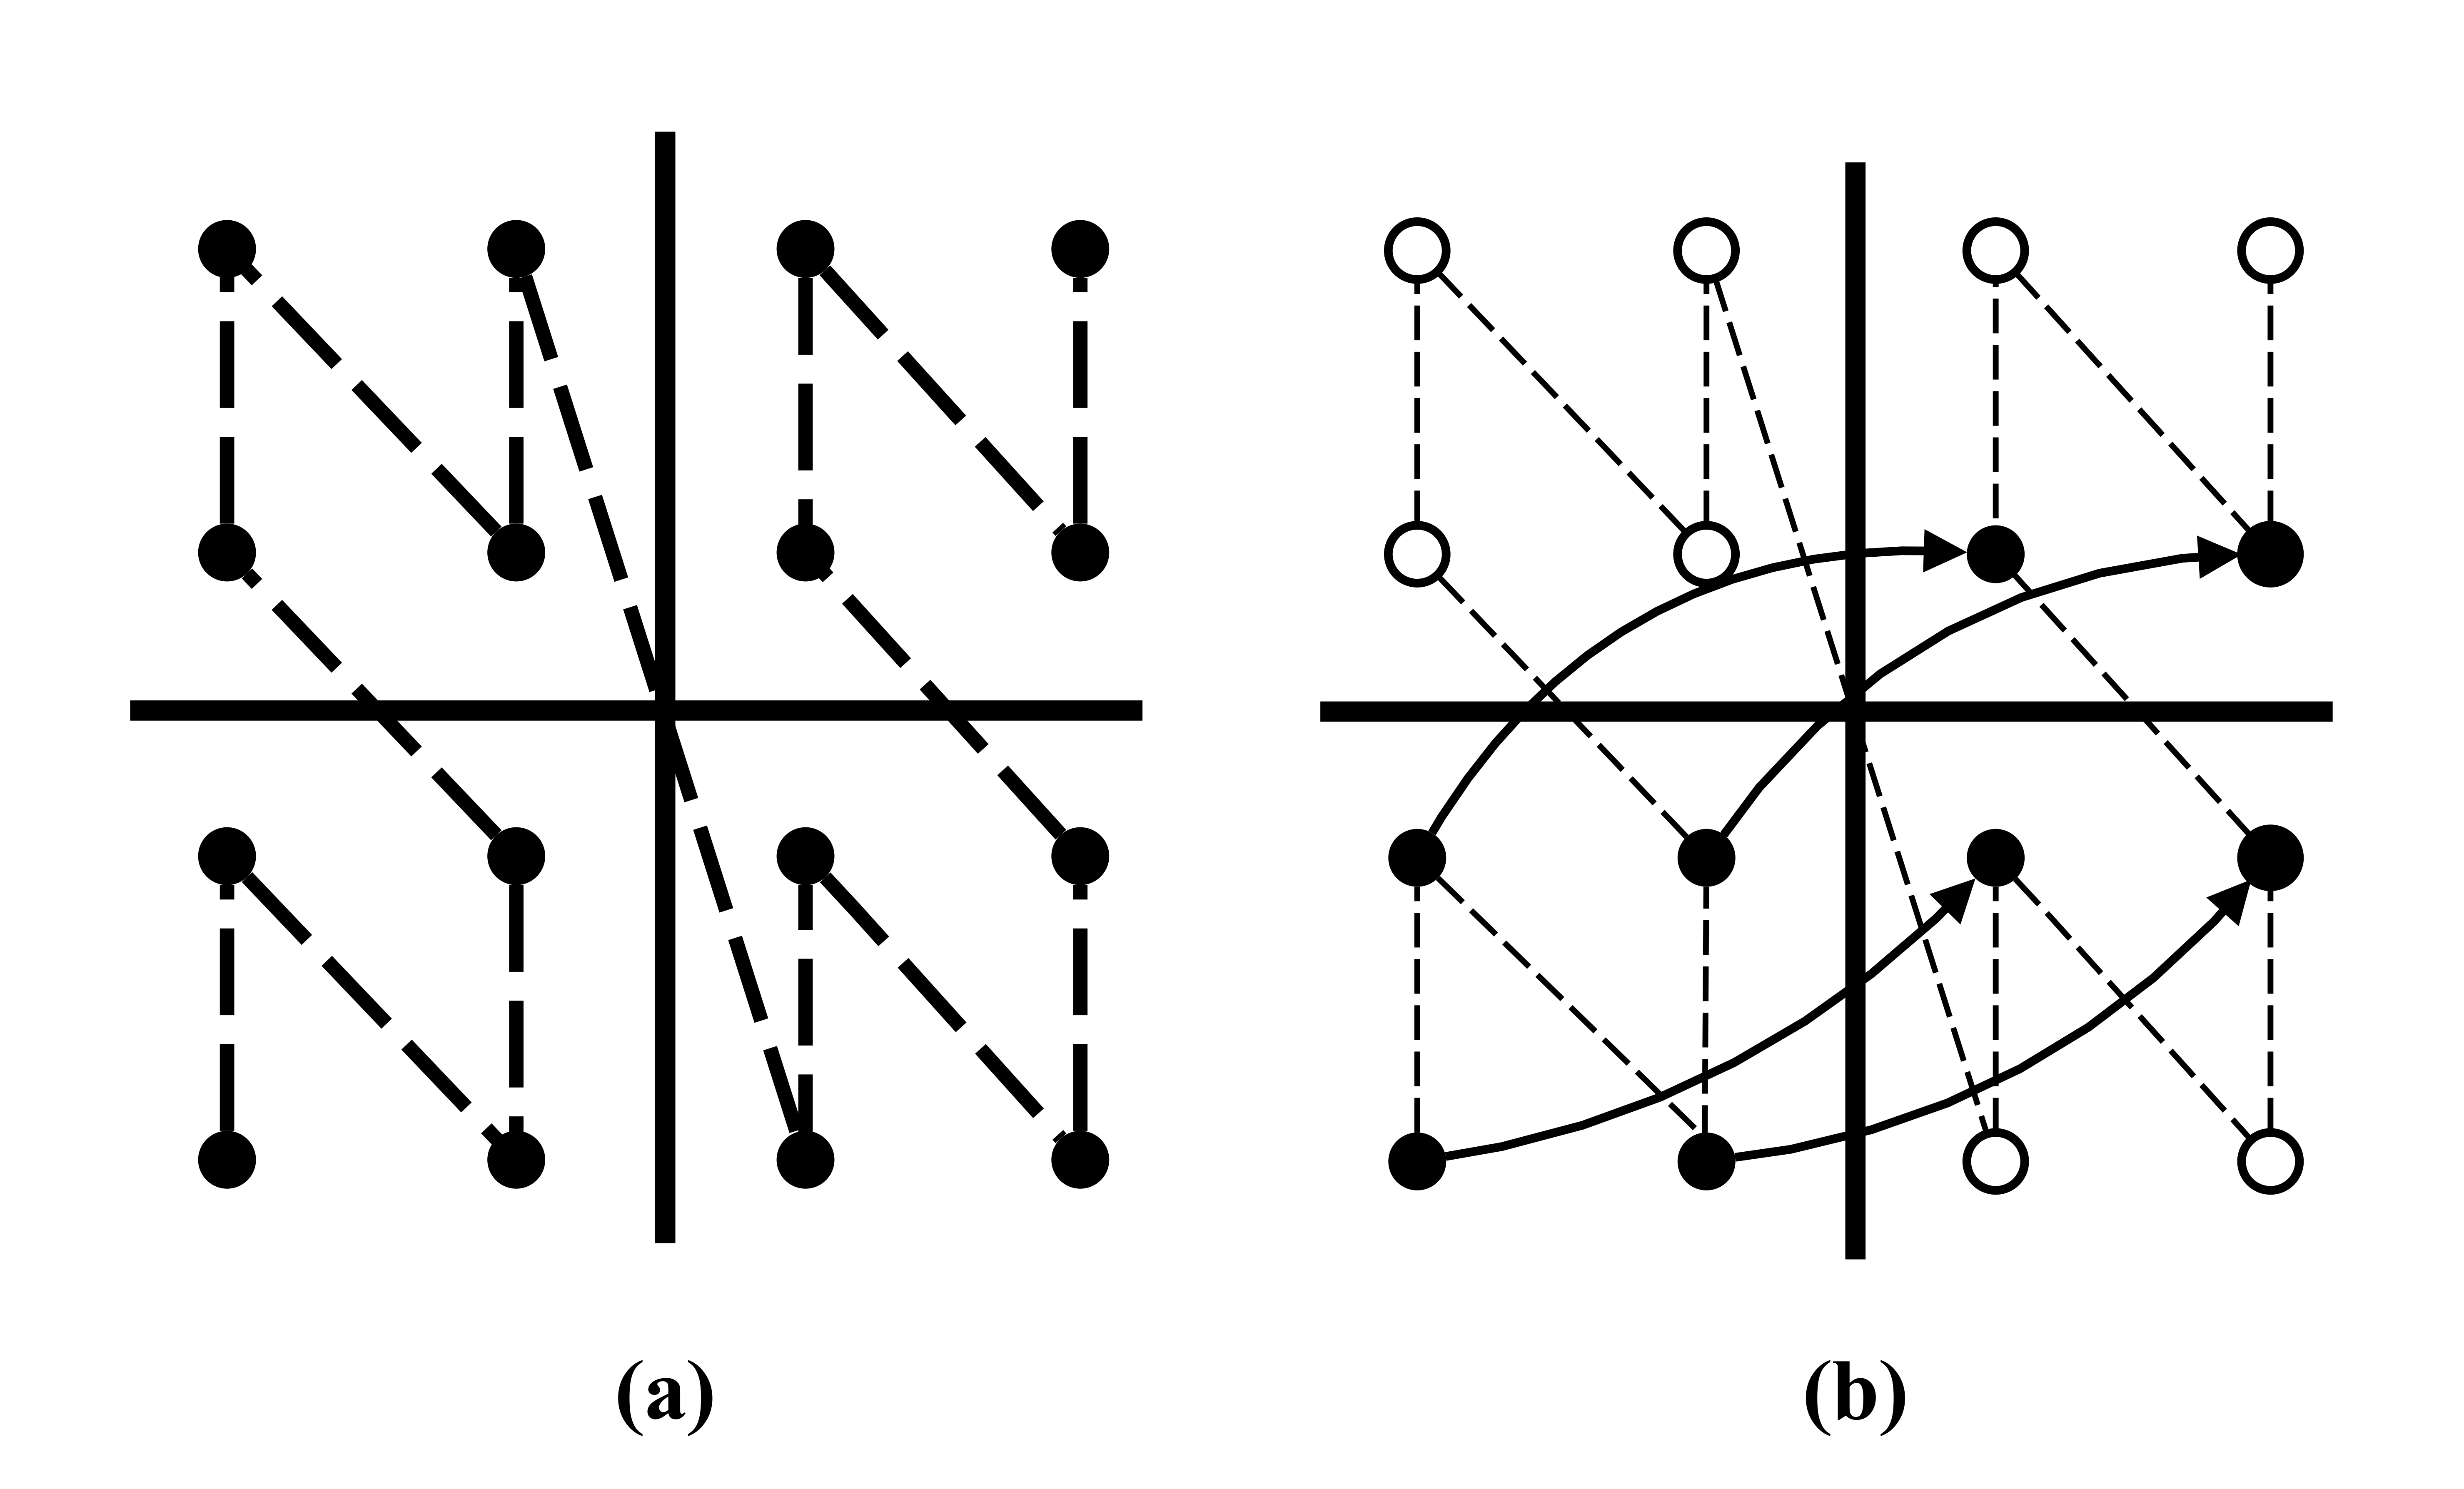
\includegraphics[width=0.5\textwidth]{figures/zorder.png}
	\caption{The $z$-order curve.}
	\label{fig:z_order}
\end{figure}

%kNN on distributed and parallel environments
Several implementations of MapReduce based $k$-NN joins algorithms have been proposed in the direction of data mining in a distributed environment. Song et al.~\cite{song2015hal} review the most efficient approaches among them, concluding that H-zkNN~\cite{zhang2012epk}, built on a SFC based approach, is significantly faster. The $k$-NN based knowledge extraction usually includes three stages, i.e. (i) data pre-processing, (ii) data partitioning and organization, and (iii) $k$-NN computation. Our work extends over the method of Zhang et al.~\cite{zhang2012epk} by additionally proposing a robust probabilistic classifier based on the MapReduce programming model, executed in a single parallel session, which achieves high prediction accuracy. We further apply this classifier on forecasting tasks in order to draw useful knowledge from huge amounts of data.

%classification, forecasting and prediction
Classification and forecasting can be performed by applying a $k$-NN classifier. It can be realized by predicting the class of a new observation and having already determined the dominant class among its nearest neighbours. Gou et al.~\cite{Gou2011jcp} present a weighted voting scheme for such classifiers, where the distance between an element and its nearest neighbours determines the weight of each neighbour, with the most weighted one determining the final class of the query element. We extend over this functionality by also computing the probability that an element has, in order to belong to each class.

Similar approaches that apply the $k$-NN classifier in the resources consumption domain, include the work of Chen et al.~\cite{chen2011aab} who used a $k$-NN classification method and labelled water data to identify water usage. However, they do not operate on huge amounts of data, while our approach lies in the field of Big Data management. Similarly, Kermany et al.~\cite{Kermany2013aam}, apply the $k$-NN classifier on low granular water consumption data, whilst this work is applied over highly granular data in a distributed and parallel environment.
